\subsection{Cut and count analysis}
\label{subsec:cutcount}

An uncategorized cut-and-count analysis is performed by applying an additional cut of $\met>320\:\GeV$ to define the signal region. The upper limits on the cross section ratio are shown in Fig.~\ref{fig:rlimits_count}. The hadronic and semileptonic channels both have roughly the same sensitivity. By combining the channels, the limits improve by about $30\%$. The limits on the cross section ratio and $M_*$ are shown in Fig.~\ref{fig:rlimits_count} and Fig.~\ref{fig:mstarlimits_count}, respectively.

\begin{figure}[htbp]
\begin{center}
  \subfigure[Hadronic]{\label{subfig:hadronic_count}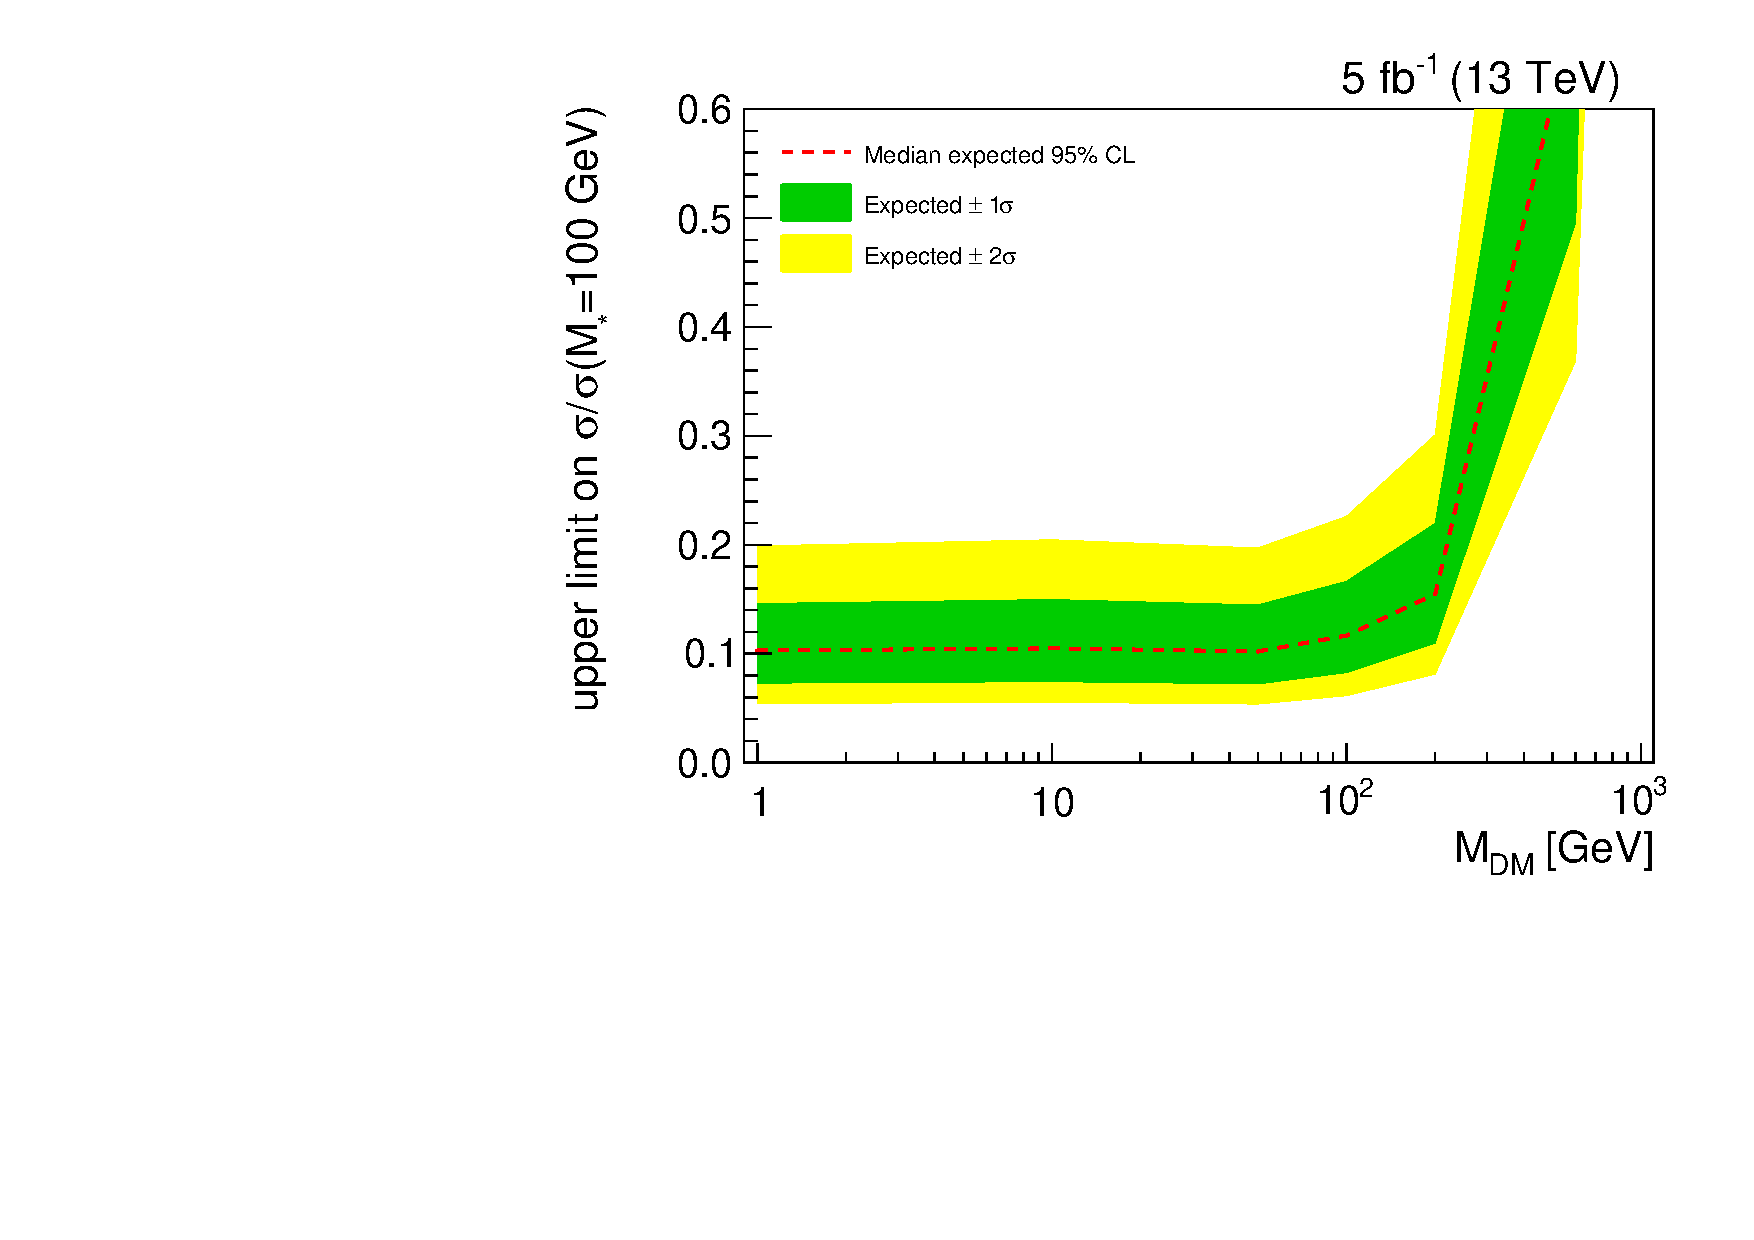
\includegraphics[width=0.32\textwidth]{figures/rLimit_hadronic_incl_count.pdf}}
  \subfigure[Semileptonic]{\label{subfig:semilept_count}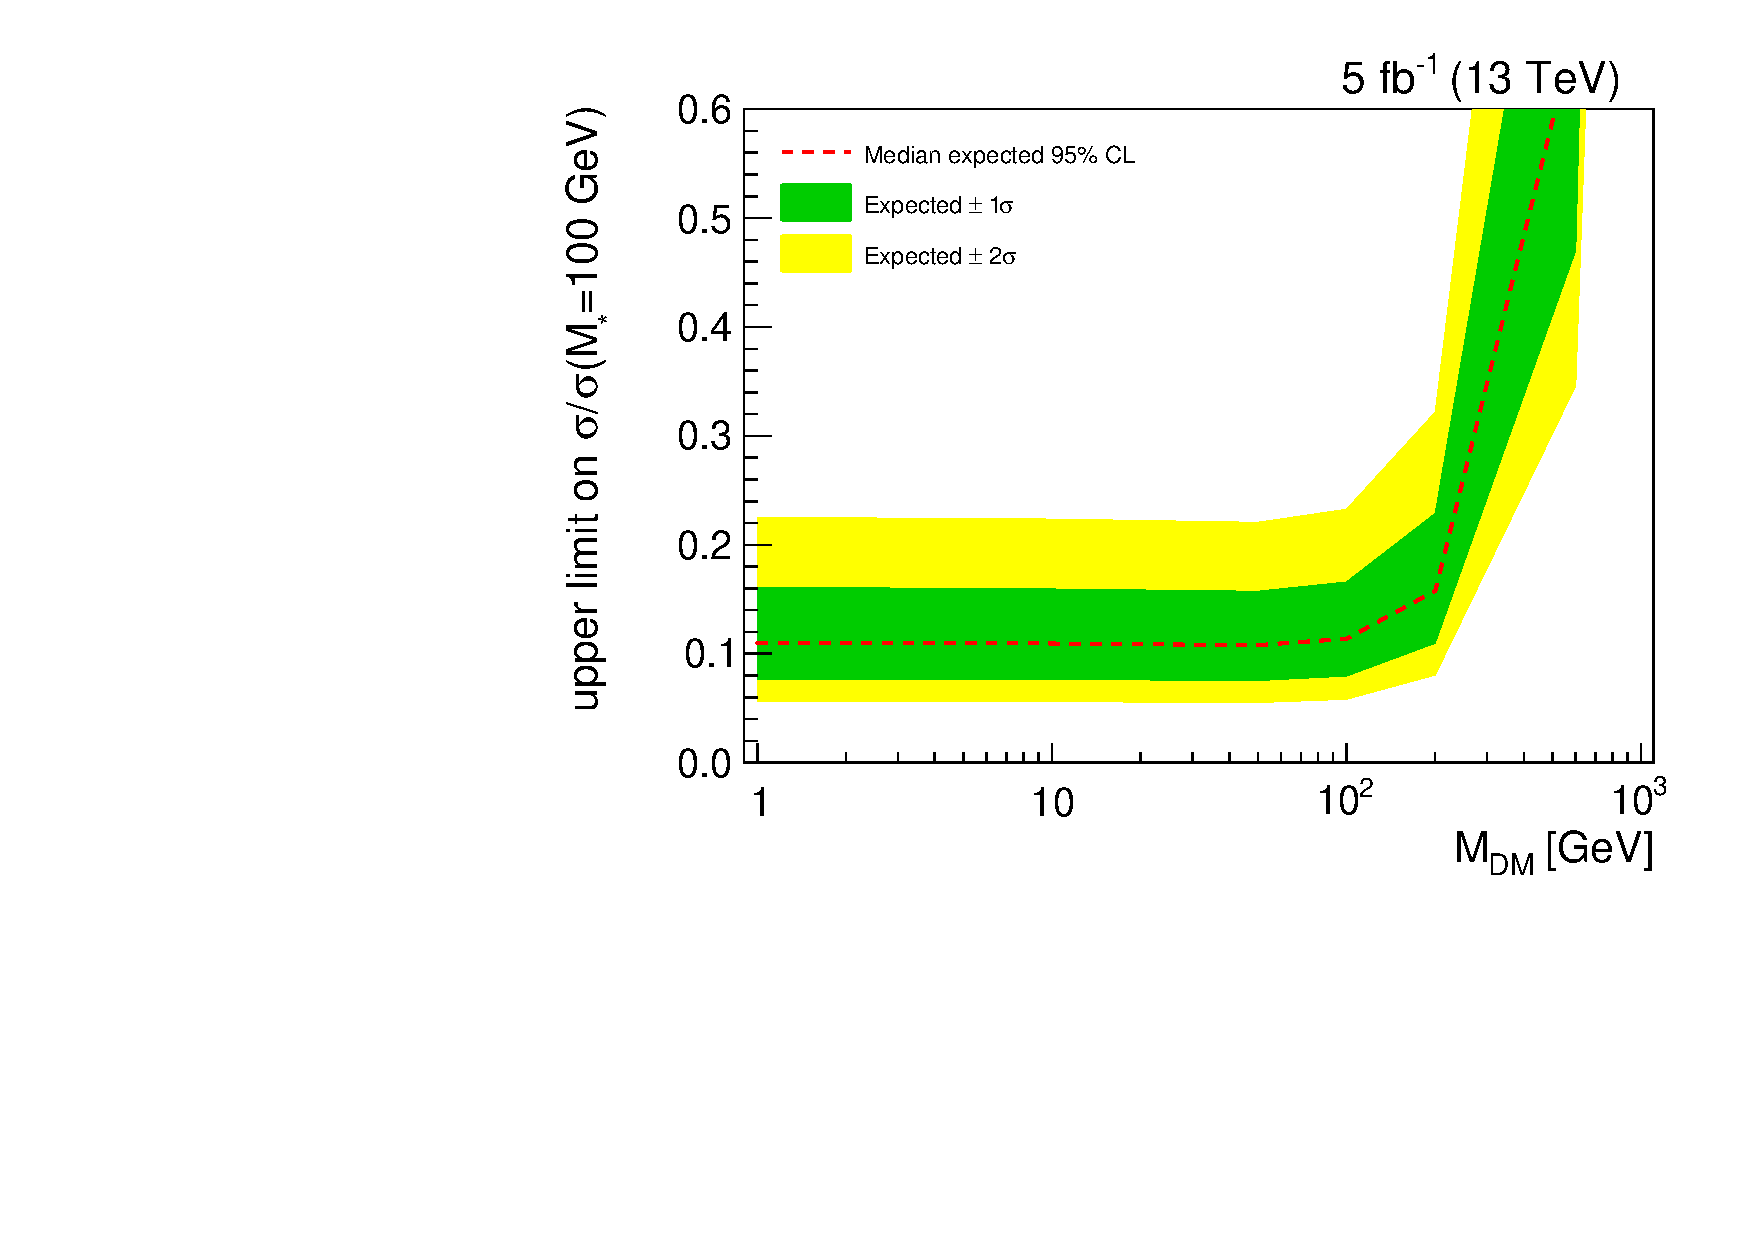
\includegraphics[width=0.32\textwidth]{figures/rLimit_semilept_incl_count.pdf}}
  \subfigure[Combined]{\label{subfig:combined_count}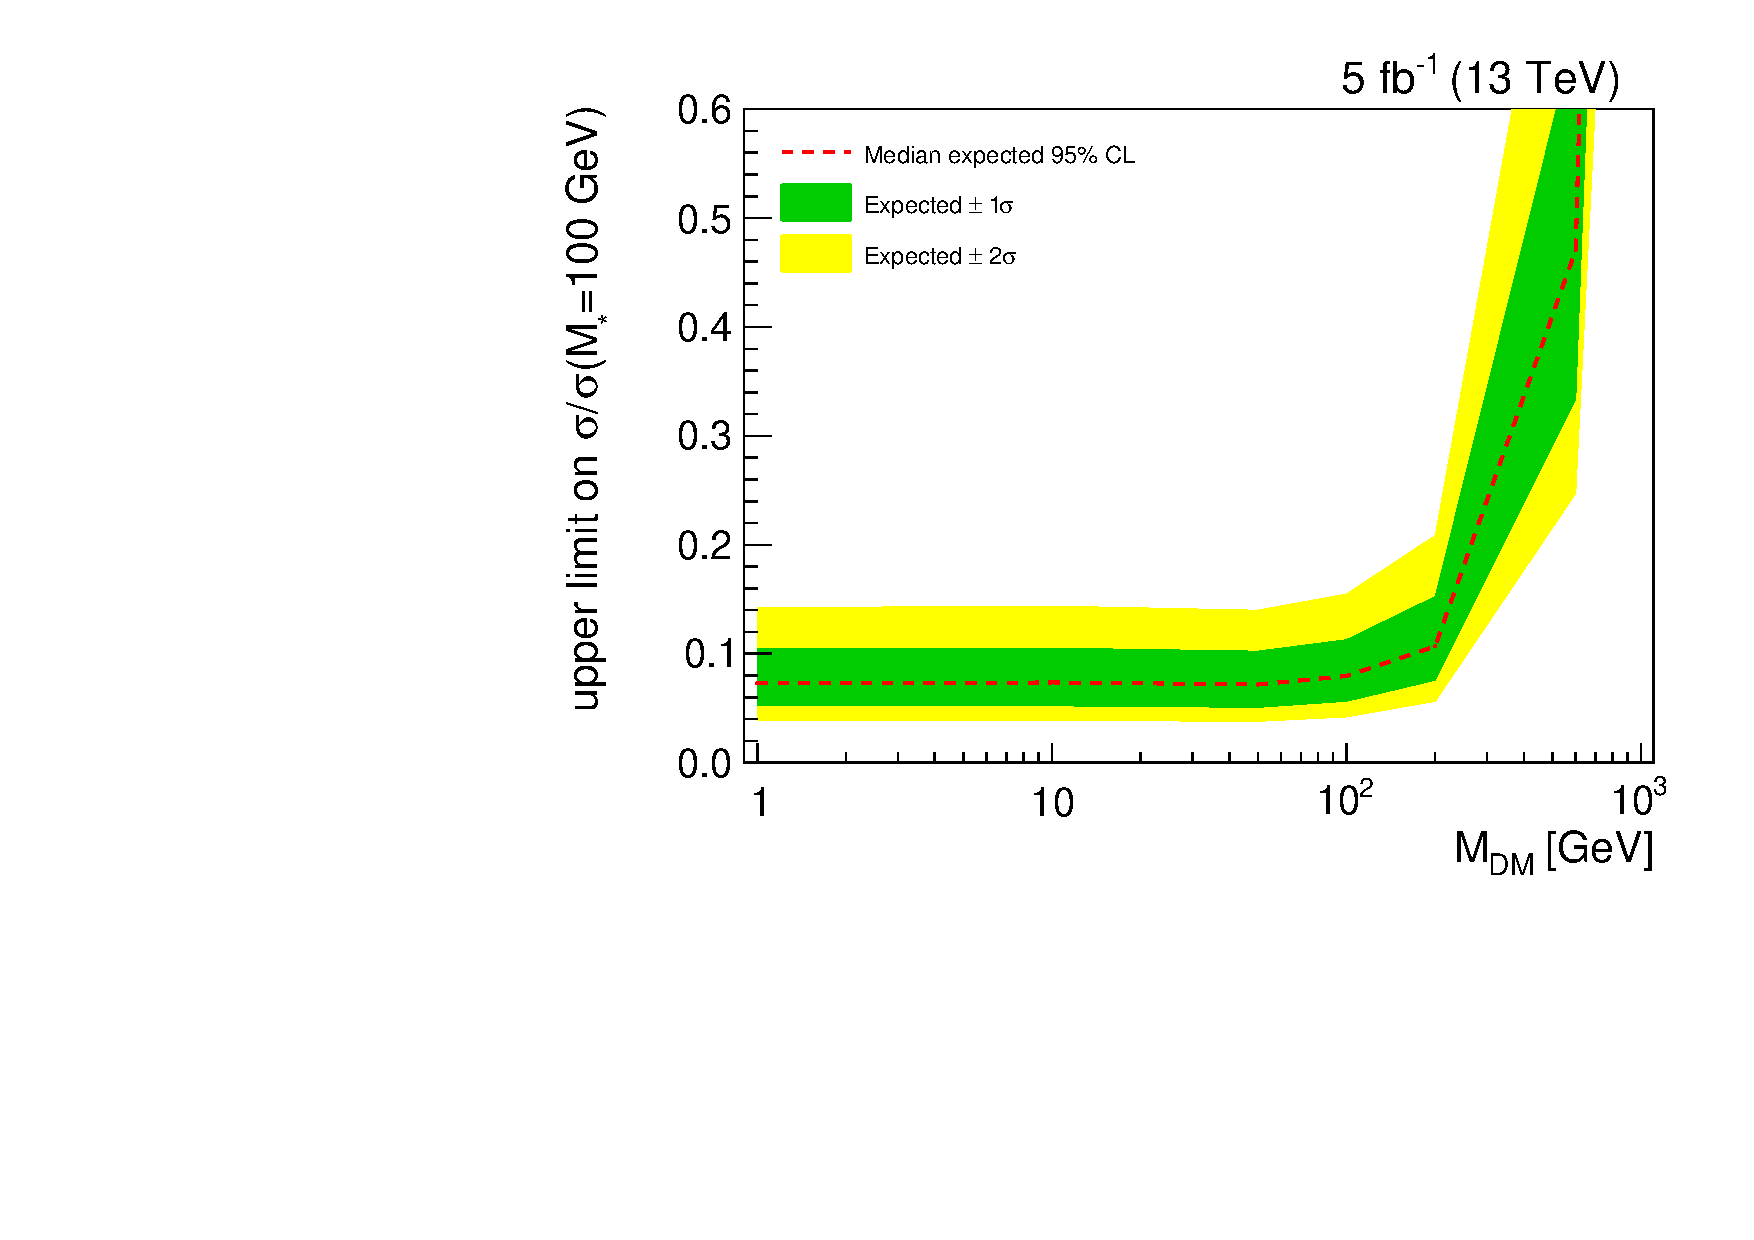
\includegraphics[width=0.32\textwidth]{figures/rLimit_incl_count.pdf}}
  \caption{Expected upper limits on the cross section ratio relative to $M_*=100\:\GeV$ for the inclusive selections: \subref{subfig:hadronic_count} hadronic channel, \subref{subfig:semilept_count} semileptonic channel, \subref{subfig:combined_count} combination of both channels.}
  \label{fig:rlimits_count}
\end{center}
\end{figure}

\begin{table}[!ht]
\centering
\begin{tabular}{|r|c|c|c|}
\hline
  $M_\chi$ $(\GeV)$ & Median & $\left[-1\sigma\, +1\sigma\right]$ & $\left[-2\sigma\, +2\sigma\right]$ \\
\hline
  $1$               & $0.1030$ & $\left[0.0730\, 0.1461\right]$ & $\left[0.0543\, 0.1990\right]$ \\
  $10$              & $0.1050$ & $\left[0.0744\, 0.1498\right]$ & $\left[0.0554\, 0.2047\right]$ \\
  $50$              & $0.1021$ & $\left[0.0723\, 0.1448\right]$ & $\left[0.0538\, 0.1971\right]$ \\
  $100$             & $0.1167$ & $\left[0.0827\, 0.1665\right]$ & $\left[0.0615\, 0.2261\right]$ \\
  $200$             & $0.1548$ & $\left[0.1097\, 0.2196\right]$ & $\left[0.0813\, 0.3010\right]$ \\
  $600$             & $0.6973$ & $\left[0.4960\, 0.9891\right]$ & $\left[0.3691\, 1.3558\right]$ \\
  $1000$            & $4.0156$ & $\left[2.8468\, 5.6963\right]$ & $\left[2.1098\, 7.8085\right]$ \\
\hline
\end{tabular}
\caption{Expected upper limits on the cross section ratio relative to $M_*=100\:\GeV$ for inclusive selection in the hadronic channel.}
\label{tab:rLimits_hadronic_count}
\end{table}

\begin{table}[!ht]
\centering
\begin{tabular}{|r|c|c|c|}
\hline
  $M_\chi$ $(\GeV)$ & Median & $\left[-1\sigma\, +1\sigma\right]$ & $\left[-2\sigma\, +2\sigma\right]$ \\
\hline
  $1$               & $0.1099$ & $\left[0.0768\, 0.1611\right]$ & $\left[0.0562\, 0.2253\right]$ \\
  $10$              & $0.1094$ & $\left[0.0764\, 0.1595\right]$ & $\left[0.0560\, 0.2237\right]$ \\
  $50$              & $0.1079$ & $\left[0.0754\, 0.1574\right]$ & $\left[0.0552\, 0.2207\right]$ \\
  $100$             & $0.1138$ & $\left[0.0795\, 0.1659\right]$ & $\left[0.0582\, 0.2327\right]$ \\
  $200$             & $0.1577$ & $\left[0.1097\, 0.2288\right]$ & $\left[0.0804\, 0.3218\right]$ \\
  $600$             & $0.6738$ & $\left[0.4703\, 0.9827\right]$ & $\left[0.3461\, 1.3784\right]$ \\
  $1000$            & $3.9531$ & $\left[2.7495\, 5.7652\right]$ & $\left[2.0152\, 8.0867\right]$ \\
\hline
\end{tabular}
\caption{Expected upper limits on the cross section ratio relative to $M_*=100\:\GeV$ for inclusive selection in the semileptonic channel.}
\label{tab:rLimits_semilept_count}
\end{table}

\begin{table}[!ht]
\centering
\begin{tabular}{|r|c|c|c|}
\hline
  $M_\chi$ $(\GeV)$ & Median & $\left[-1\sigma\, +1\sigma\right]$ & $\left[-2\sigma\, +2\sigma\right]$ \\
\hline
  $1$               & $0.0728$ & $\left[0.0521\, 0.1044\right]$ & $\left[0.0384\, 0.1423\right]$ \\
  $10$              & $0.0737$ & $\left[0.0522\, 0.1052\right]$ & $\left[0.0389\, 0.1438\right]$ \\
  $50$              & $0.0718$ & $\left[0.0508\, 0.1024\right]$ & $\left[0.0379\, 0.1400\right]$ \\
  $100$             & $0.0796$ & $\left[0.0564\, 0.1129\right]$ & $\left[0.0420\, 0.1548\right]$ \\
  $200$             & $0.1069$ & $\left[0.0757\, 0.1525\right]$ & $\left[0.0564\, 0.2085\right]$ \\
  $600$             & $0.4707$ & $\left[0.3337\, 0.6715\right]$ & $\left[0.2473\, 0.9238\right]$ \\
  $1000$            & $2.7422$ & $\left[1.9339\, 3.9008\right]$ & $\left[1.4407\, 5.3396\right]$ \\
\hline
\end{tabular}
\caption{Expected upper limits on the cross section ratio relative to $M_*=100\:\GeV$ for combined hadronic and semileptonic channel.}
\label{tab:rLimits_count}
\end{table}

\begin{figure}[htbp]
\begin{center}
  \subfigure[Hadronic]{\label{subfig:hadronic_countm}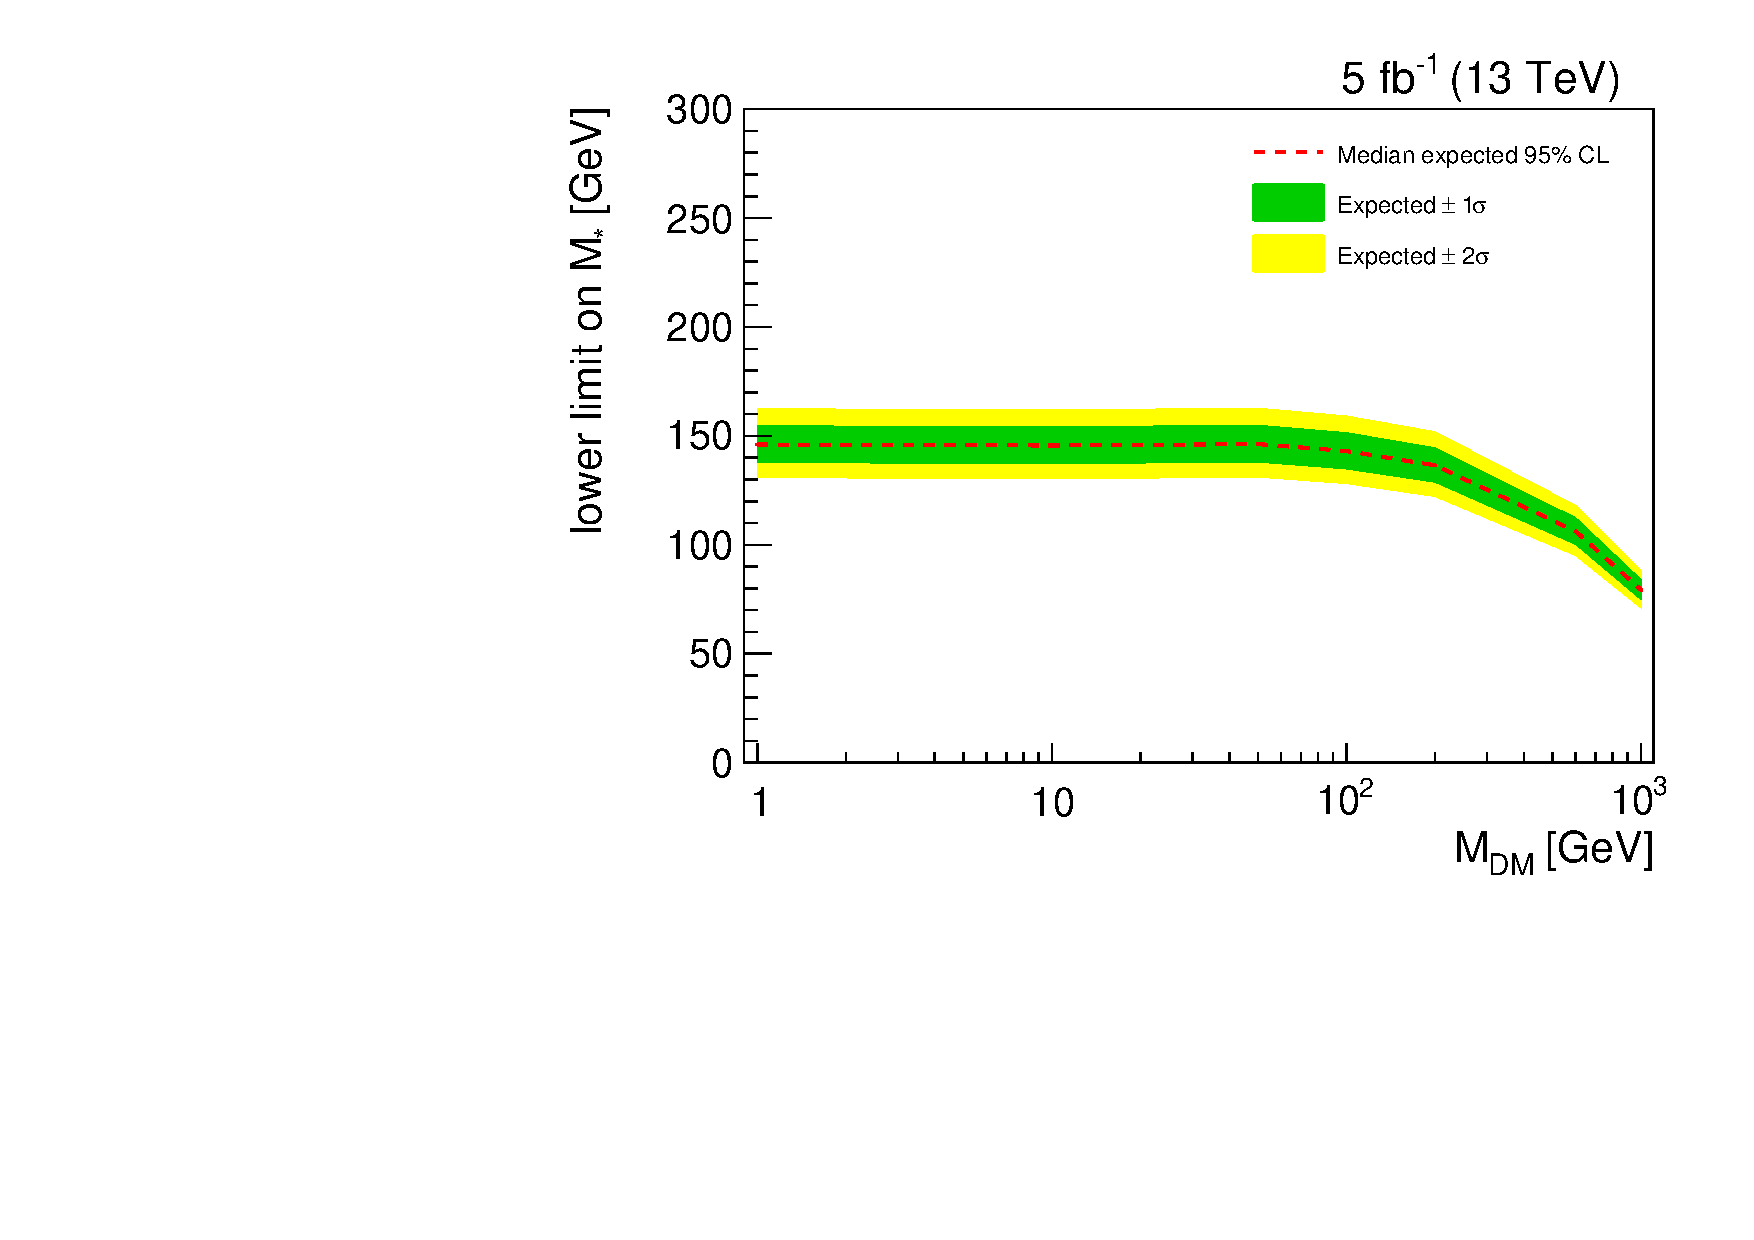
\includegraphics[width=0.32\textwidth]{figures/mstarLimit_hadronic_incl_count.pdf}}
  \subfigure[Semileptonic]{\label{subfig:semilept_countm}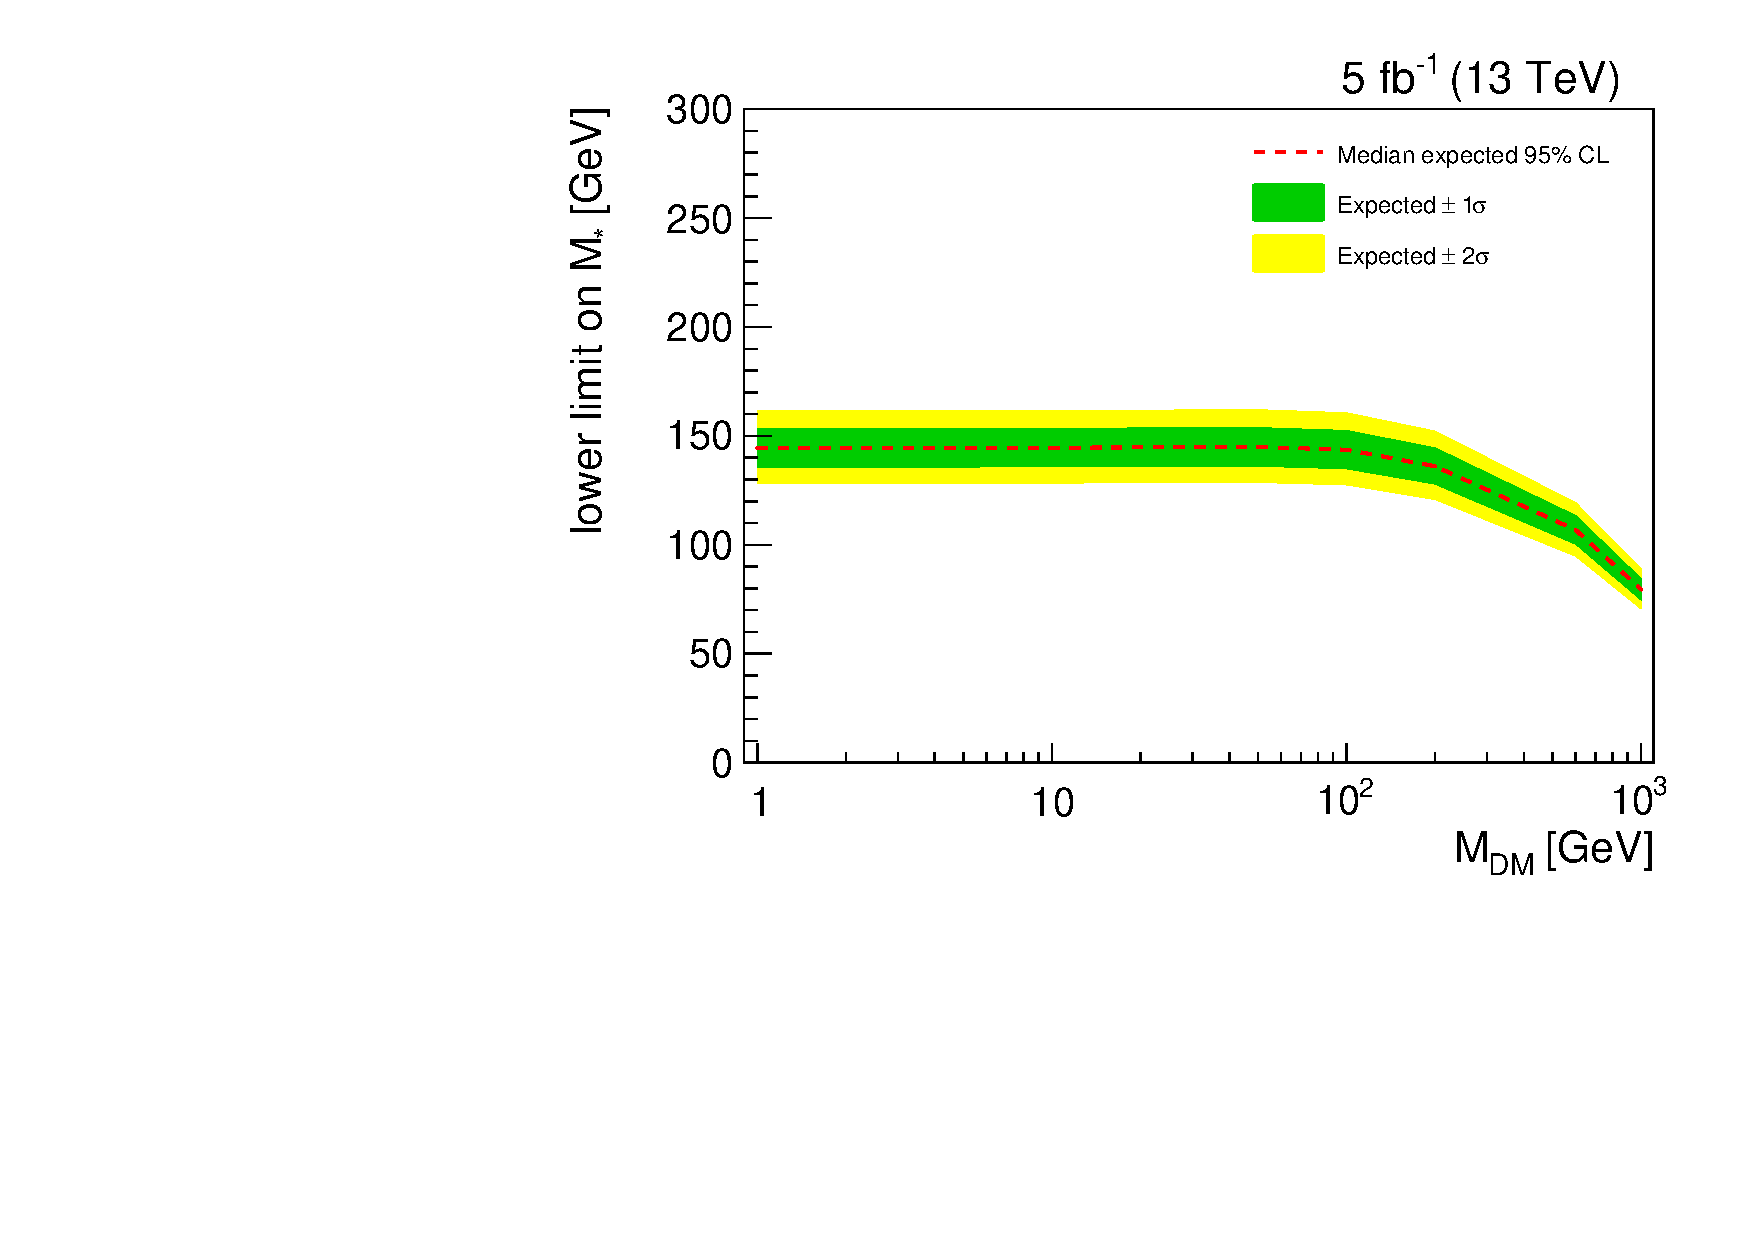
\includegraphics[width=0.32\textwidth]{figures/mstarLimit_semilept_incl_count.pdf}}
  \subfigure[Combined]{\label{subfig:combined_countm}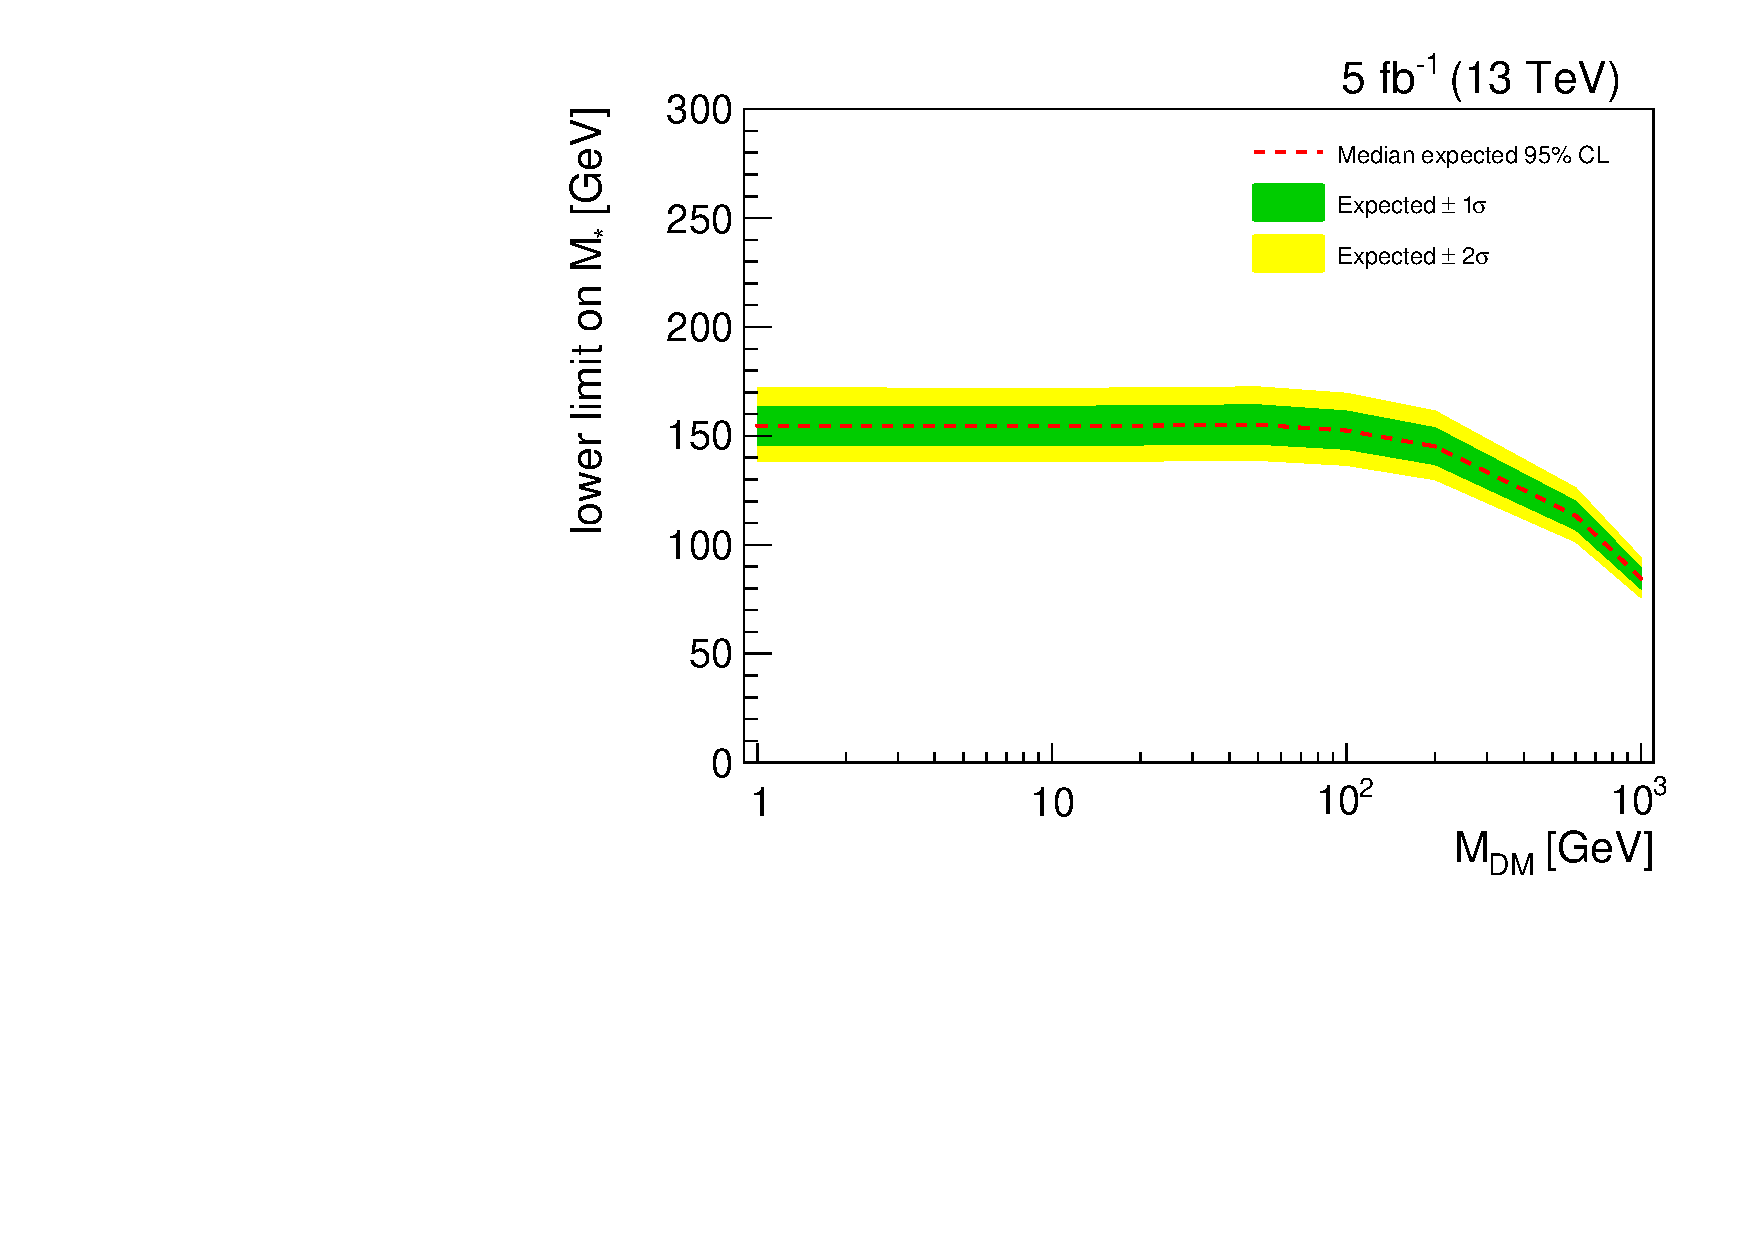
\includegraphics[width=0.32\textwidth]{figures/mstarLimit_incl_count.pdf}}
  \caption{Expected lower limits on $M_*$ for the inclusive selections: \subref{subfig:hadronic_countm} hadronic channel, \subref{subfig:semilept_countm} semileptonic channel, \subref{subfig:combined_countm} combination of both channels.}
  \label{fig:mstarlimits_count}
\end{center}
\end{figure}
